%!TEX root = ../Physik I.tex

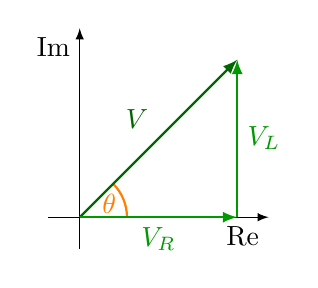
\begin{tikzpicture}[>=latex,scale=2]
	\begin{scope}
		\draw[->] (0,-.2) -- (0,1.2) node[below left]{Im};
		\draw[->] (-.2,0) -- (1.2,0) node[below left]{Re};
	\end{scope}
	
	
	\begin{scope}[thick]
		\draw[color=orange] (.3,0) arc (0:45:.3cm) node[below, xshift=-.05cm]{$\theta$};
		\draw[->,color=green!40!black] (0,0) -- (1,1) node[pos=.5,above left]{$V$};
		\draw[->,color=green!60!black] (1,0) -- (1,1) node[pos=.5,right]{$V_L$};
		\draw[->,color=green!60!black] (0,0) -- (1,0) node[pos=.5,below]{$V_R$};
	\end{scope}
\end{tikzpicture}